To access the web application, navigate to a domain and directory that publicly serves the web page. An example of this could be: \url{https://scratchy.cs.umu.se:8000/app/}. All functionality of the web application is (or rather should be) fairly self-explanatory and intuitive. A short description and explanation will be given for each component that has been implemented so far.
\subsection{Using the interface}
This section describes how to use the interface and how to interact with it.
\subsubsection{Start view}
%figure 1
\begin{figure}[h]
\centering
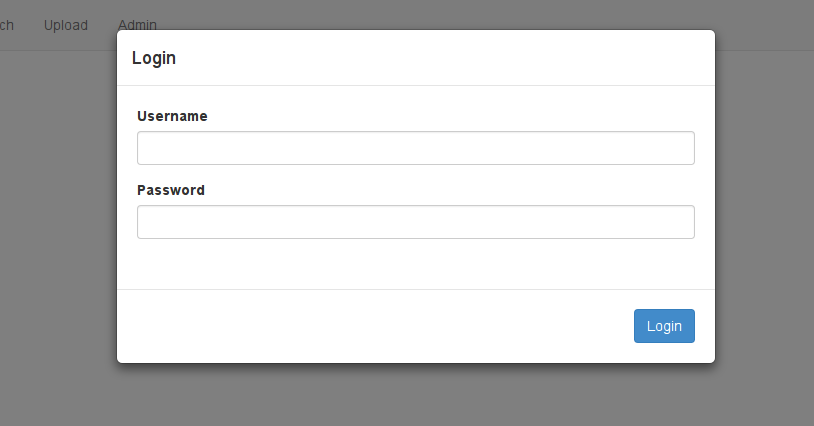
\includegraphics[width=0.75\textwidth]{web/manual/web_login.png}
\caption{\label{fig:web_search_login} The login pop-up window.}
\end{figure}
When first entering the web page, the login pop-up window in \refer{fig:web_search_login} is shown and the user will have to enter their username and password to gain access to the application.

%figure 2
\begin{figure}[h] 
\centering
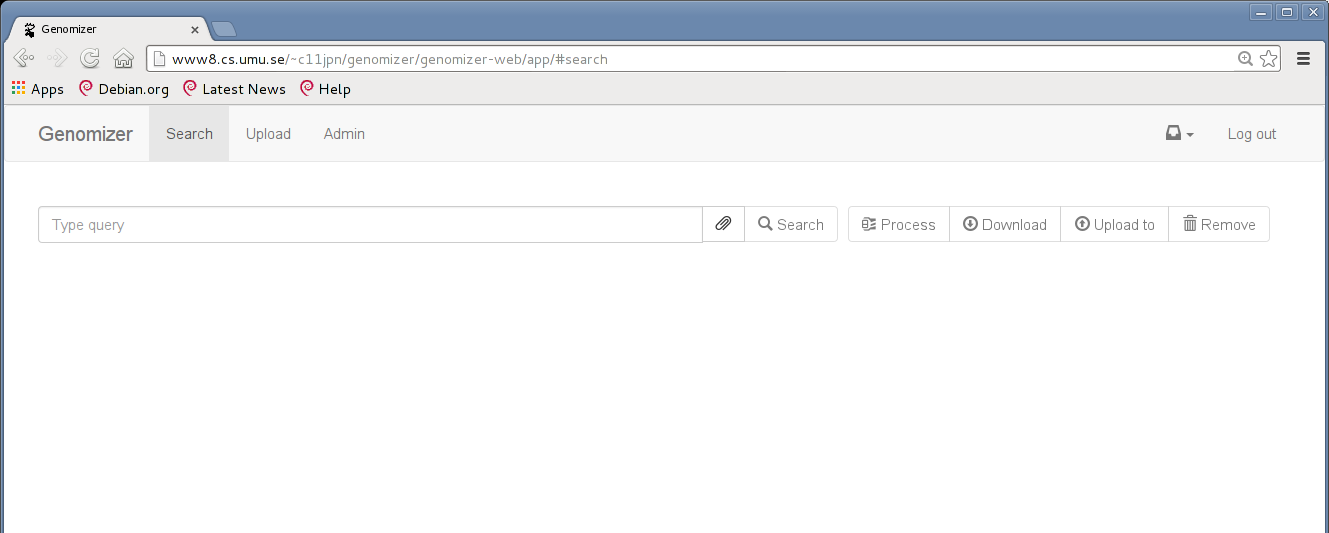
\includegraphics[width=1\textwidth]{web_search_welcome.png}
\caption{\label{fig:web_search_welcome} The start view of the web page.}
\end{figure}

When the user has logged in, the user is taken to the search page as shown in \refer{fig:web_search_welcome}.

The navigation bar at the top has a number of buttons to the left and two buttons to the right with the following functionality:
\begin{itemize}
	\item Clicking the “Genomizer” logo takes the user right back to the start view.
	\item The “Search” button will bring up the search view where the user can enter search strings to be sent to the server, and view search results.
	\item The “Upload” button will bring up the upload view where the user can select files to be uploaded and input annotation to a new experiment.
	\item The “Process” button will bring up the process view where the user can select an experiment to process.
	\item The “Administration” button will bring up the admin view where the user can handle genome releases and annotations.
    \item The inbox icon on the left side opens a dropdown list which displays the statuses of files currently being processed.
    \item The “Log out” button will log out the user.
\end{itemize}
This navigation bar is persistent through all sub pages and can easily be accessed.

\subsubsection{Search view}

In the search view, below the navigation bar, a “search-and-functionality” bar is visible. There is a search field and there are seven buttons that are explained below, starting with the left-most button: 

\begin{itemize}
	\item ”Query builder”, represented by a paperclip, brings up a query builder, shown in \refer{fig:web_search_queryBuilder}, that helps unexperienced users construct a valid query used for searching experiments. Just select a value in the three fields and press add. The correct pubmed-styled query will be shown in the search field and the three query fields will be reset so the user can add more things to search for in their query.
	\item “Search” searches for the query in the search field. 
	\item “Process” processes the selected files.
    \item “Convert” converts the selected files. This feature is demonstrated further in section \ref{sssec:convertView}.
    \item “Upload to” opens the upload view with the selected experiments selected where the user can upload new files to an already existing experiment.
    \item “Remove” opens a new view where the files which are going to be deleted are presented along with a confirmation dialog that the user really wants to delete those files and experiments.
\end{itemize}

\begin{figure}[h]
\centering
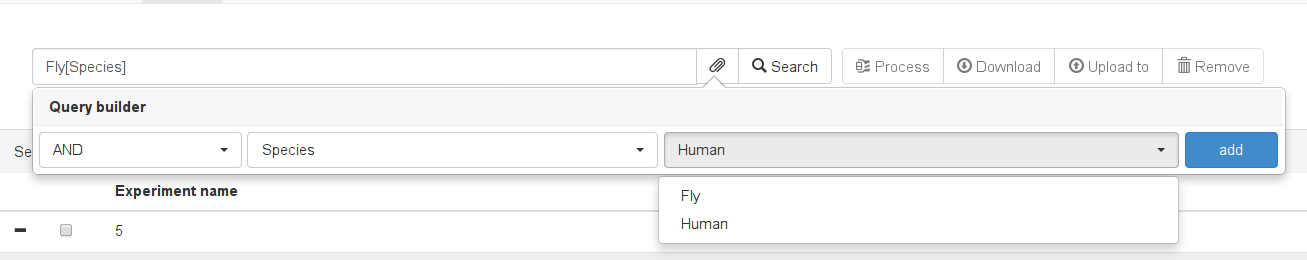
\includegraphics[width=1\textwidth]{web_search_queryBuilder.png}
\caption{\label{fig:web_search_queryBuilder}The query builder.}
\end{figure}

When first entering the search view, only the query builder button and the search button are clickable. The rest of the buttons become clickable once the user selects experiments or files. To search, the user can either write a pubmed style query (for example: \textit{”Fly[Species]”} to search for every experiment with ”Fly” as value of the annotation ”Species”) or use the query builder. When clicking the search button, a loading screen is shown. The experiment data is displayed once it has been retrieved from the server.

%figure x3
\begin{figure}[h]
\centering
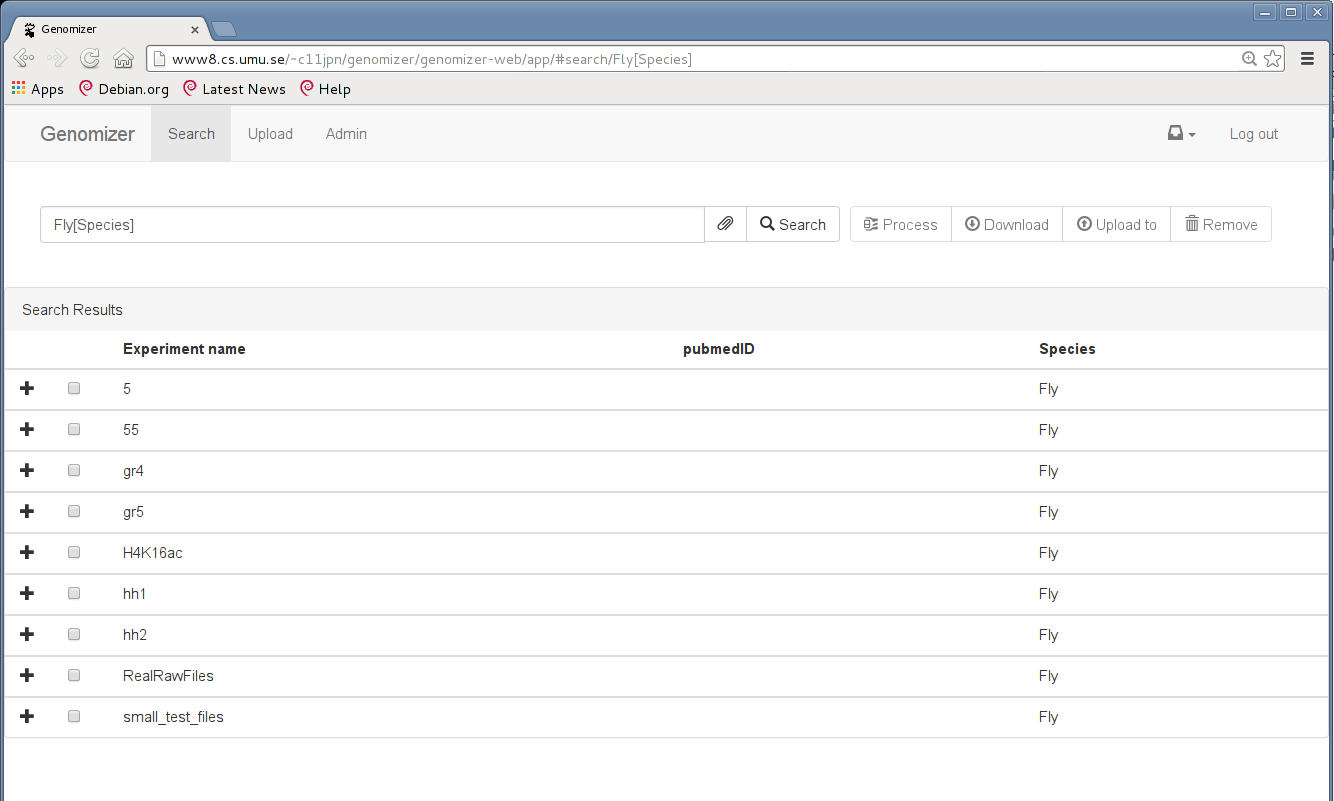
\includegraphics[width=1\textwidth]{web_search_searchTab.png}
\caption{\label{fig:web_search_searchTab}The search tab after searching for \textit{“Fly[Species]”}.}
\end{figure}

The view in \refer{fig:web_search_searchTab} is shown when the user has searched for the query \textit{”Fly[Species]”}. The displayed list contains all experiments returned from the search and a header on top with all annotation types. Every experiment can be expanded by clicking it to show the file types it contains. Each file type can be further expanded to show all files of that type in the experiment. Every file and experiment has a checkbox next to it that is used to select it. In \refer{fig:web_search_searchResult}, an experiment called \class{Ratiotest} and its contained collection of \class{raw} files have been expanded. Furthermore, the files \class{test.fastq} and \class{test2.fastq} have been selected. These files can now, for example, be processed or removed by using the buttons in the “search-and-functionality” bar.

%figure x4
\begin{figure}[h]
\centering
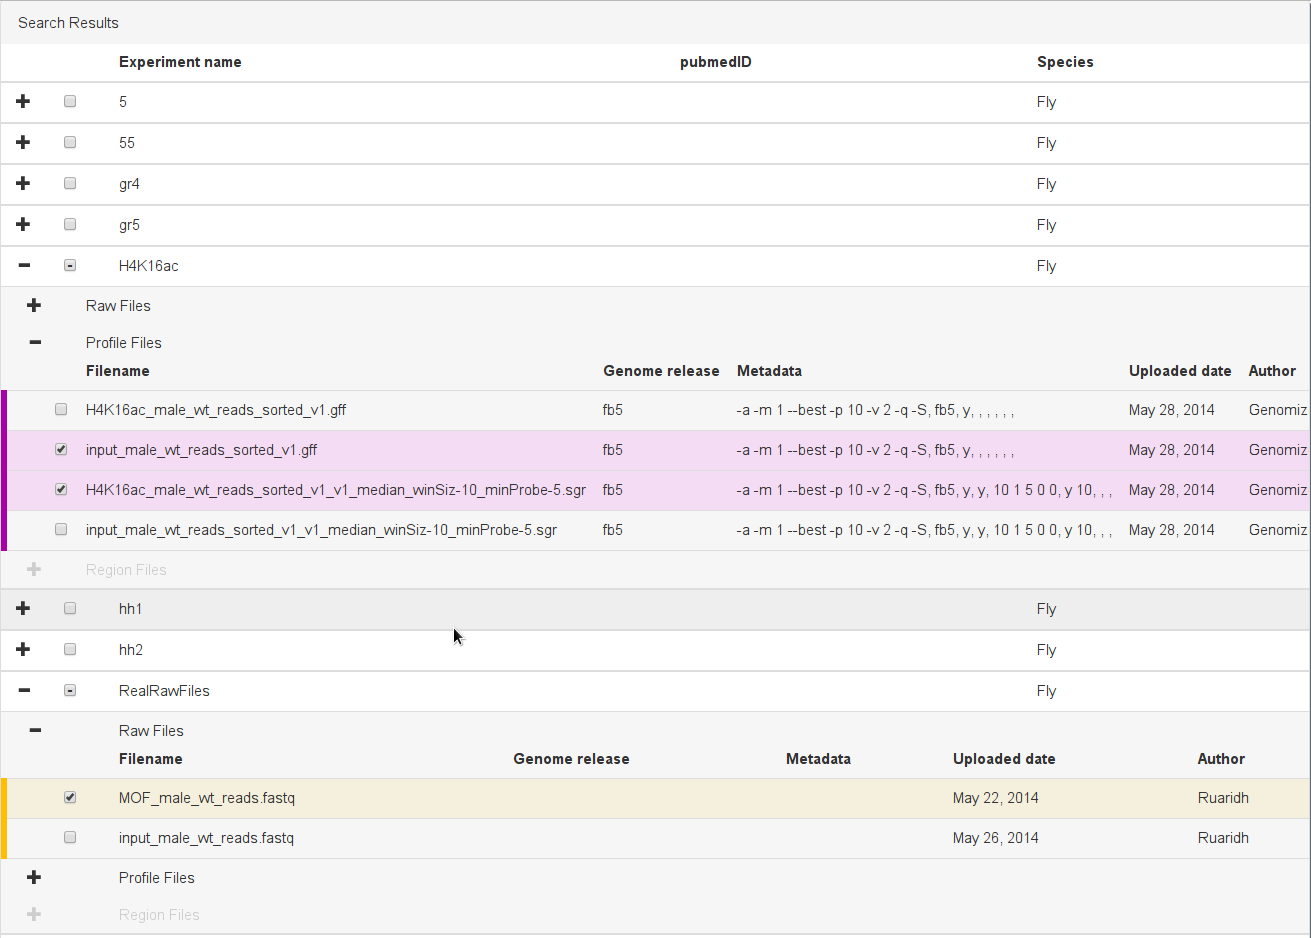
\includegraphics[width=1\textwidth]{web_search_searchResult.png}
\caption{\label{fig:web_search_searchResult}The search results table zoomed in, displaying the information of a \class{raw} file after having expanded an experiment.}
\end{figure}

If no experiments match the search query, the Search Results table will be empty stating “No search results found”.

\pagebreak
\subsubsection{The processing view}
%figure X6

\FloatBarrier

If the user wants to process files from an experiment they first have to enter the search view and search for the experiment in which they wish to process files. Check the box for the experiment and then click the process button (\refer{fig:web_process_step1}).
\begin{figure}[h!]
\centering
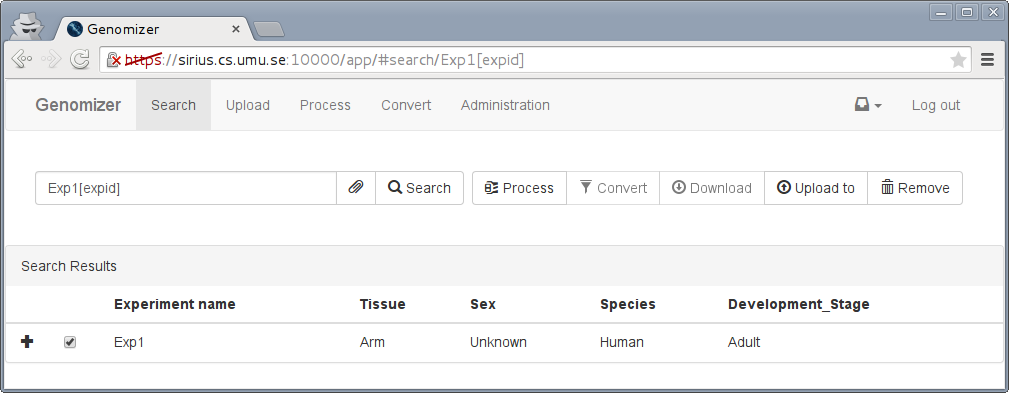
\includegraphics[width=1\textwidth]{web_manual_process_step2.png}
\caption{\label{fig:web_process_step1}Selected Exp1.}
\end{figure}
\begin{figure}[h!]
\centering
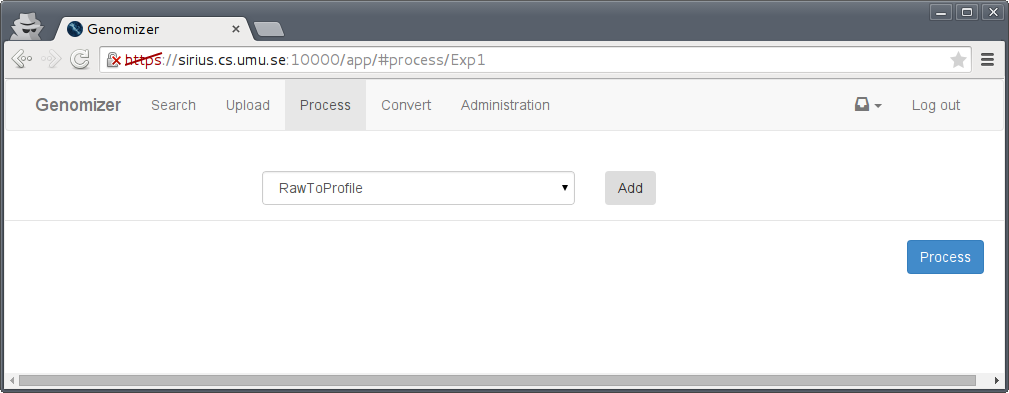
\includegraphics[width=1\textwidth]{web_manual_process_step3.png}
\caption{\label{fig:web_process_step2}The process view opened with Exp1 selected.}
\end{figure}
When the process view is opened choose which process step you want to do in the dropdown list and then press the add button (\refer{fig:web_process_step2}).
\begin{figure}[h!]
\centering
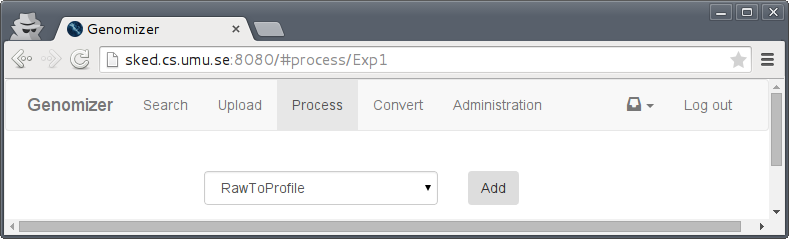
\includegraphics[width=1\textwidth]{web_manual_process_step4.png}
\caption{\label{fig:web_process_step3}Scrollbar which shows the different process steps.}
\end{figure}
To add a new file to the selected process step press the ''+''
 button (\refer{fig:web_process_step3}).
 \begin{figure}[h!]
\centering
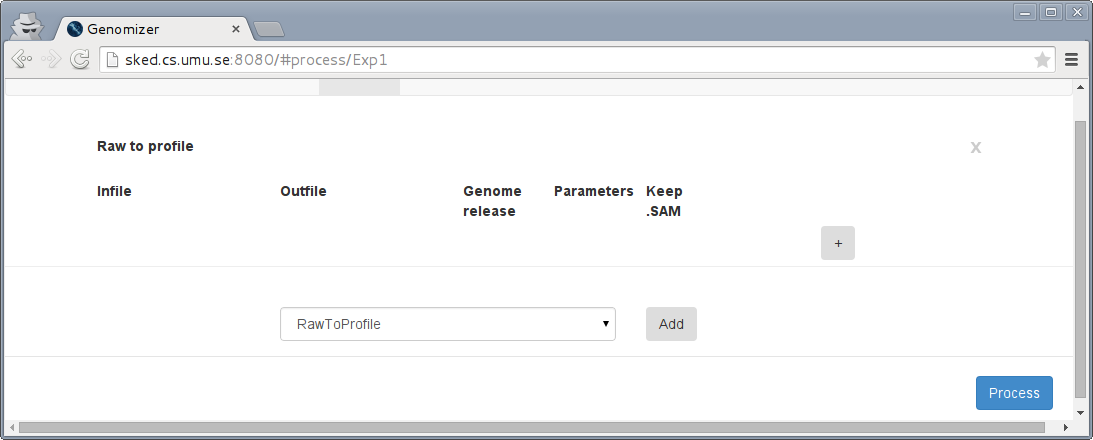
\includegraphics[width=1\textwidth]{web_manual_process_step5.png}
\caption{\label{fig:web_process_step4}Process view after a process step has been selected.}
\end{figure}
After pressing the ''add'' button the view will now show a new set of processing options. The ''Infile'' dropdown list chooses which file is going to be processed. ''Outfile'' is used to set the name for the new processed file. ''Genome release'' sets which genome release to use for the process and ''Parameters'' sets which parameters to be used. If the user wants the \class{.sam} file to be saved the ''Keep .SAM'' box has to be checked (\refer{fig:web_process_step4}).
\begin{figure}[h]
\centering
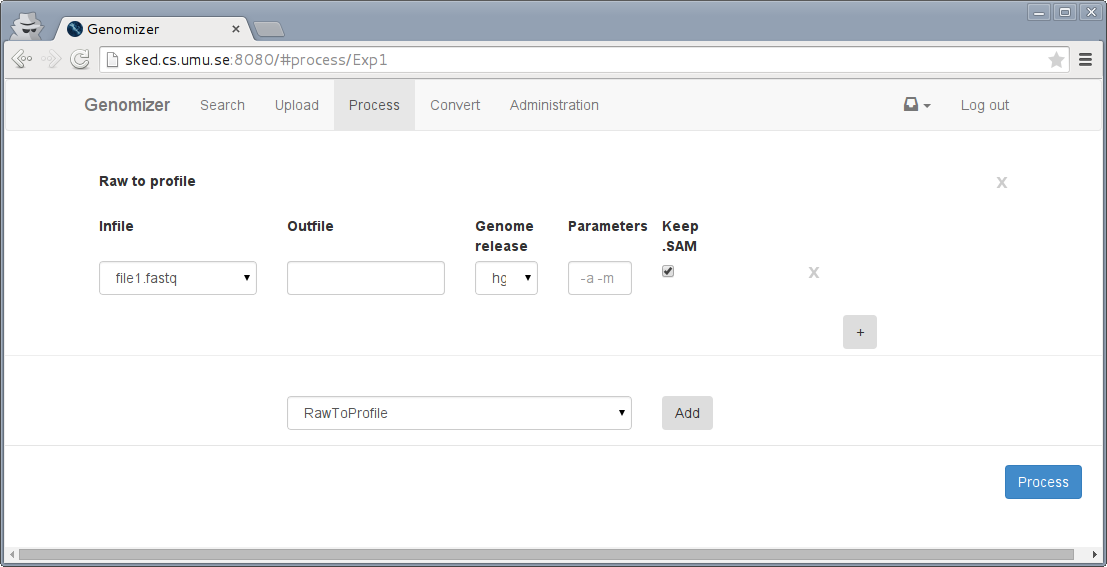
\includegraphics[width=1\textwidth]{web_manual_process_step6.png}
\caption{\label{fig:web_process_step5}Process view after adding a file for a process step.}
\end{figure}
To start processing simply press the ''Process'' button (\refer{fig:web_process_step5}).

%WAAAAAAAAAAAAAAAAAAAAAAAAAAAAAAAAAAAAAAAAAAAAAAAAAAAAAAT


\pagebreak



\subsubsection{The convert view} \label{sssec:convertView}

The web application allows conversion between a number of file formats which both are of profile type. More specifically, the user may convert any of the file formats \class{.sgr, .wig, .bed} and \class{.gff} to either \class{.wig} or \class{.sgr}, with the exception that a file cannot be converted to the same file format.

\begin{figure}[h]
\centering
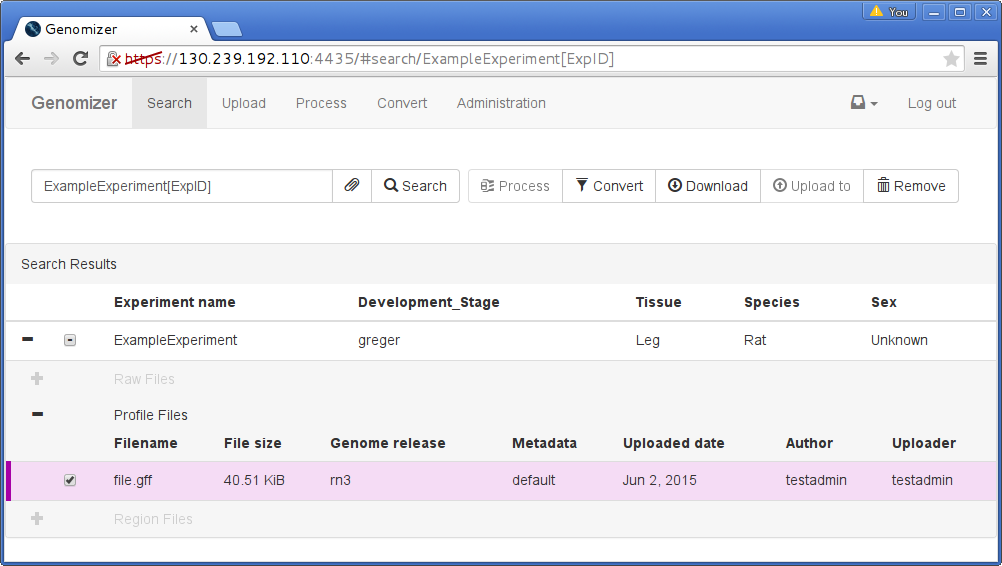
\includegraphics[width=1\textwidth]{web_convert_searchExp.png}
\caption{\label{fig:web_convert_searchExp}Selecting a file to convert.}
\end{figure}

Assume that there is an experiment \class{ExampleExperiment} which contains a profile file \class{file.gff}. Then the experiment will show up in the search view, see \refer{fig:web_convert_searchExp}, when typing ”ExampleExperiment[ExpID]” as search query and then clicking the search button. If the user wants to convert \class{file.gff} to a new file of format \class{.wig} called \class{file.wig}, the following steps can be taken:
\begin{itemize}
	\item From the view in \refer{fig:web_convert_searchExp}, select \class{file.gff} by clicking in its checkbox.
	\item Click the “Convert” button next to the search text field.
	\item The user will now be taken to the convert view shown in \refer{fig:web_convert_convertView}.
	\item Select \class{file.gff} by clicking on it.
	\item Mark the \class{.wig} checkbox in “Convert to” and click the “Convert” button.
\end{itemize}

\begin{figure}[h]
\centering
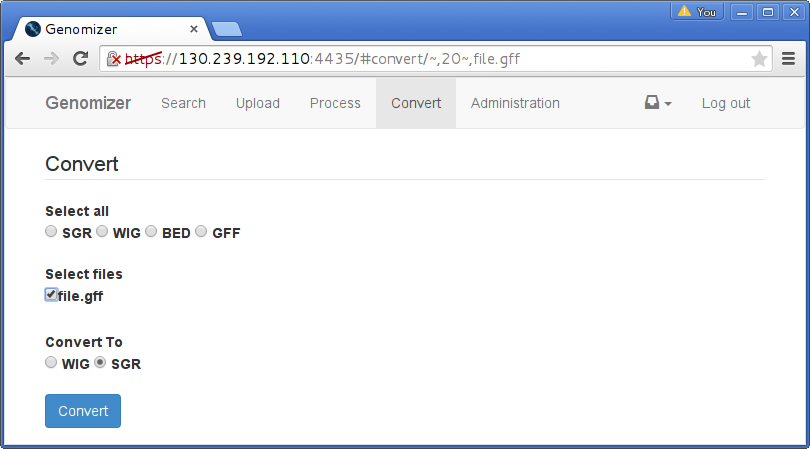
\includegraphics[width=1\textwidth]{web_convert_convertView.png}
\caption{\label{fig:web_convert_convertView}The convert view.}
\end{figure}

The file conversion will now start on the server. Once the conversion is done, the user will be able to see \class{file.wig} listed together with the old file \class{file.gff} when searching for the experiment.

If multiple files are selected for conversion, all of them will appear as a list in the convert view. If the user quickly wants to select all files of a specific file format, for example all \class{.wig} files, the GFF option can be marked in “Select all”. Then all files in the list of the format \class{.wig} will automatically be selected.

\subsubsection{The remove pop-up window}
\begin{figure}[h]
\centering
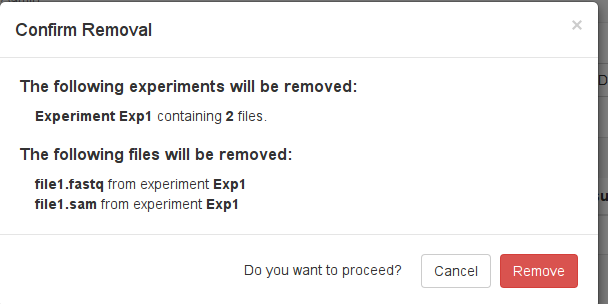
\includegraphics[width=0.8\textwidth]{web/manual/web_remove.png}
\caption{\label{fig:web_remove_removeFiles}The remove pop-up window.}
\end{figure}
\FloatBarrier
When the remove button is pressed the pop-up window in \refer{fig:web_remove_removeFiles} is shown displaying which files and experiments will be removed when the remove button is pressed.


\subsubsection{The process status dropdown}
\begin{figure}[h]
\centering
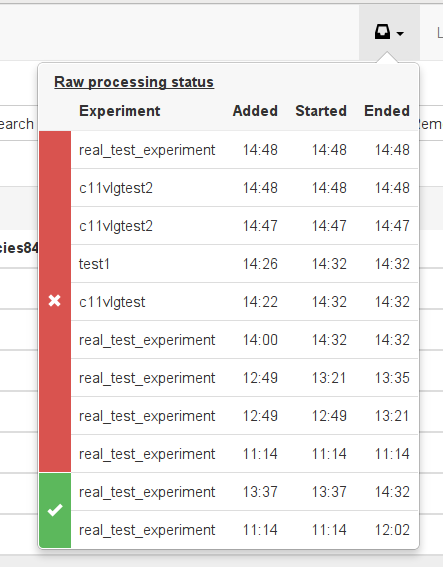
\includegraphics[width=0.5\textwidth]{web_processStatus_withData.png}
\caption{\label{fig:web_processStatus_withData}The process status dropdown.}
\end{figure}
\FloatBarrier
When pressing the inbox icon, a dropdown is shown as in \refer{fig:web_processStatus_withData} displaying the status of experiments currently being processed. There are four different statuses a processing can have, all grouped into colors: Waiting (yellow), Running (blue), Complete (green) and Failed (red). For example, in the figure, the two bottom experiments are complete and the rest have failed. If there are no experiments being processed, the dropdown will simply display “No process status available”.


\subsubsection{The upload view}

%figure X7
\begin{figure}[h]
\centering
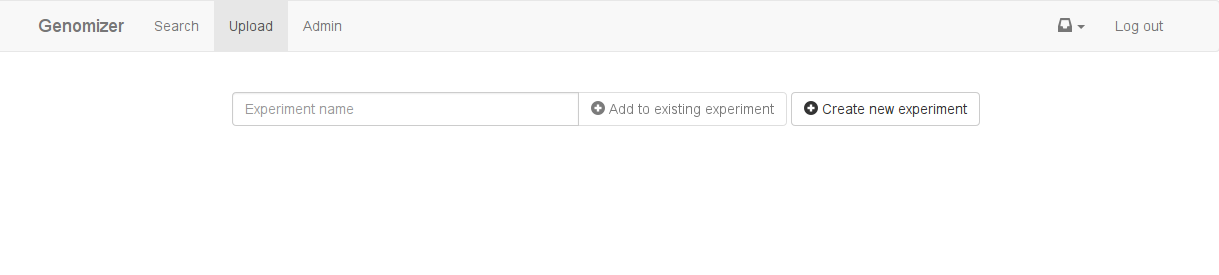
\includegraphics[width=1\textwidth]{web_upload_uploadView.png}
\caption{\label{fig:web_upload_uploadView}The upload view.}
\end{figure}

When the user clicks the upload tab in the navigation bar, the view in \refer{fig:web_upload_uploadView} will appear. The user has the option to create a new and fresh experiment or to load an existing experiment by entering its experiment name. 

%figure X8
\begin{figure}[h]
\centering
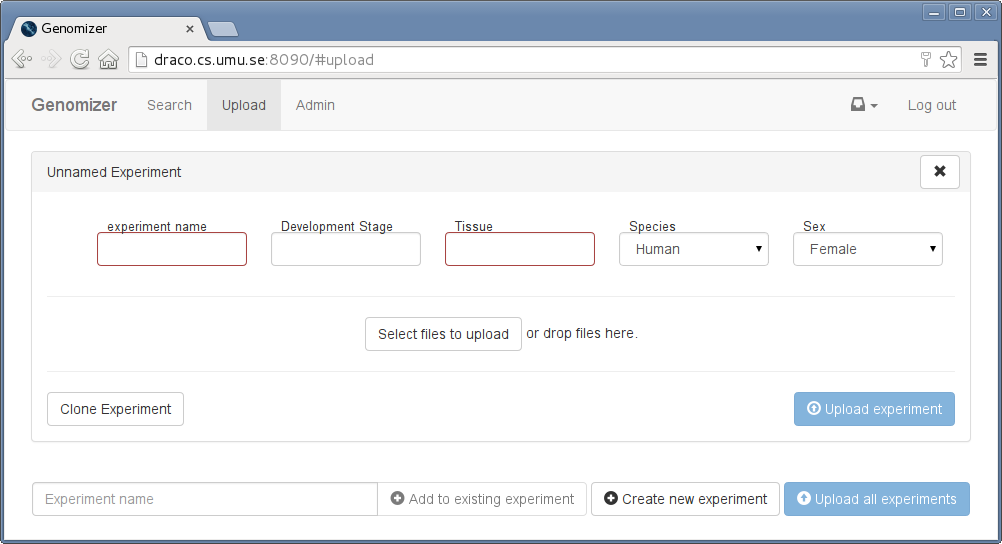
\includegraphics[width=1\textwidth]{web_upload_newExperiment.png}
\caption{\label{fig:web_upload_newExperiment}Creating a new experiment.}
\end{figure}

After clicking the “Create new experiment” button, the view in \refer{fig:web_upload_newExperiment} will appear. Here the user can input the annotations for the experiment through either freetext fields or dropdown lists. If a freetext field has a red border around it, that annotation is required and the experiment cannot be uploaded before all required fields have been filled in and at least one file has been added.

The user can create more experiments by clicking the “Create new experiment” button and a new empty experiment will be placed below the first experiment. The user can also clone an experiment by clicking the “Clone Experiment” button. What happens in this case, is that the every filled-in annotations gets copied to the new experiment.

To add files to the experiments the user can browse for local files and upload them by clicking the “Select files to upload” button. The user will only see file types that have to do with experiments but have the ability to search for all file types. There is also a way of adding files to the experiment by dragging them from a file browser and dropping them onto the experiment “drag and drop”.

An experiment can only contain two \class{raw} files and if the user tries to upload more a message with this information will appear and the experiment cannot be uploaded before the extra \class{raw} file/s is removed. 

To add files to a existing experiment the user types the name of the experiment in the field next to the “Upload to existing experiment” and clicks the button. If the experiment exists on the server it will appear in the experiment view the same way that a new experiment is shown. The annotations of an existing experiment cannot be changed from this view and if there are files already in this experiment they cannot be manipulated. Adding new files to existing experiments works the same way as to a new experiment.

%figure X9
\begin{figure}[h]
\centering
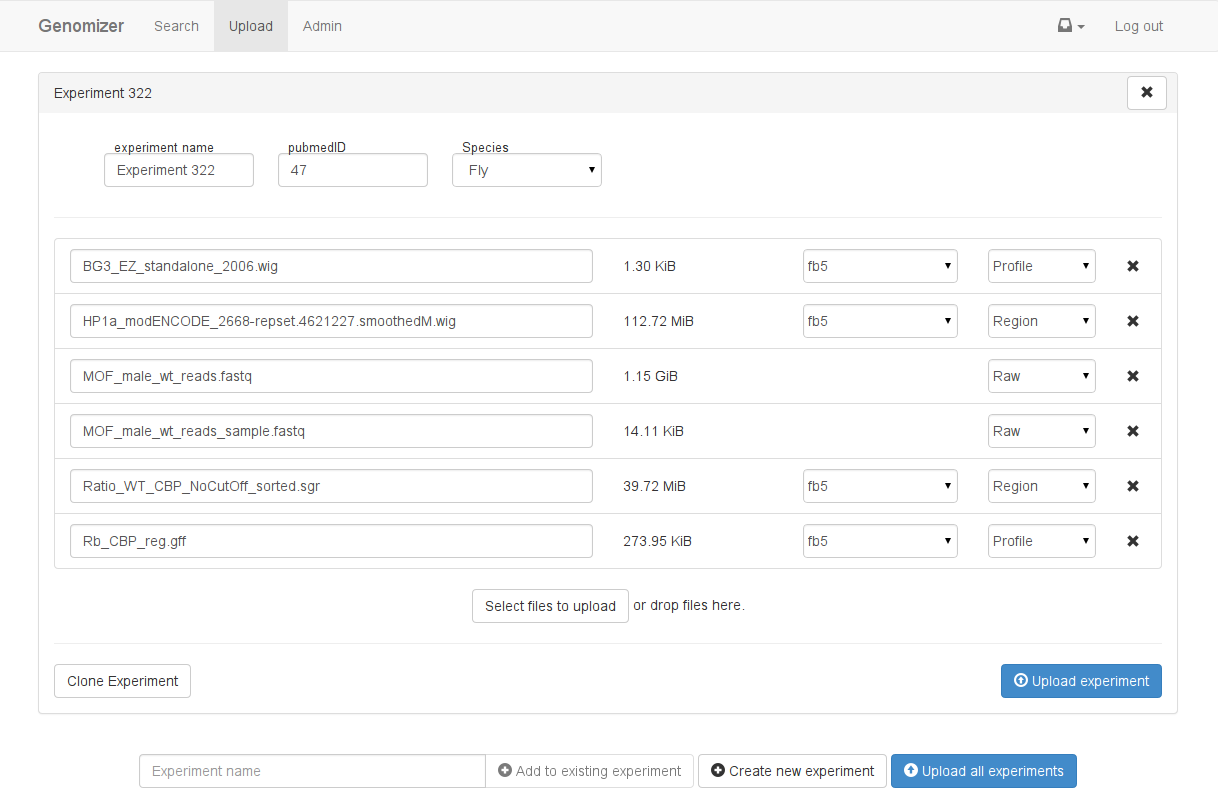
\includegraphics[width=1\textwidth]{web_upload_fileUpload.png}
\caption{\label{fig:web_upload_fileUpload}Files selected for upload.}
\end{figure}
 
When the user selects files, they will appear below the annotations as in \refer{fig:web_upload_fileUpload}. The file name is displayed in a text field on the left side of the file view. Next to the file name is a box that shows the size of the selected file. On the right side there is an option to select what type of file is being uploaded and an option to remove the file from the experiment. If the file type is either \class{profile} or \class{region}, there is an option to select what genome release the file is mapped to. The file type option will automatically be filled in with a guessed value depending on the file ending as follows: \class{.fastq} files are considered \class{raw} and all other formats (\class{.sgr, .wig, .gff}) are interpreted as \class{profile}.

When the user is done selecting files, filling in annotations and clicks the “Upload experiment” button the experiment view will be minimized showing only the name of the experiment and the progress bar of the files being uploaded. When the progress bar is done it turns green and now the experiment with all the files have been uploaded to the server. The user also has a way of uploading several experiments at the same time by clicking “Upload all experiments”. 

\subsubsection{System administration view}

This part of the web application is only accessible if the user has administrator rights. It is integrated with the rest of the web user interface and accessible through the “Administration” tab. The administrator can through this site see all annotations, add new annotations and edit existing ones.

The start page of this section has a “Create New Annotation” button, a list of existing annotations in the database and an edit button per existing annotation. The view looks like in \refer{adm__web_annotationView}. 

\begin{figure}[h]
 \addImage{web_SysadminAnnotationView.jpg}
 \caption{The start page for the administrator in the web client.}
 \label{adm__web_annotationView}
\end{figure}

For each annotation in the annotations list, an “Edit” button is available. When pressed, it will take the user to a page in which they can edit the selected annotation to change its name and what values the dropdown list will have if it is not a freetext field (see \refer{adm_web_editView}). 

\begin{figure}[h]
 \addImage{web_SysadminEditView.jpg}
 \caption{The edit annotation view.}
 \label{adm_web_editView}
\end{figure}
In the edit page, the admin can see the attributes of the chosen annotation and is able to delete the chosen annotation or change the information of it. The “Delete Annotation” button will delete the whole annotation, and for that reason two pop-up windows will appear to confirm that the administrator is sure of the action.

The administrator can change the list of annotation values. The site will automatically check whether something is added, removed or both and sends a request to change the annotation values to the server when the “Update Annotation” button is clicked.

If the admin clicks on the “Create new annotation” button from the admin start page, another view will open with the following structure:
\begin{itemize}
 \item Annotation Name
 \subitem Admin can enter a name for the annotation.
 
 \item Annotation Types
 \subitem Yes/No/Unknown - creates a dropdown list with those three options.
 \subitem freetext - creates an annotation where the users will be able to enter anything.
 \subitem Dropdown list - will enable a fourth field enabling the admin to enter which items that this list will contain.
 
 \item Forced Annotation
 \subitem Admin can choose if the new annotation should be required by users to enter. 
\end{itemize}

A Create Annotation will, if all necessary information has been entered, result in a popup (see \refer{adm_web_createPopup}) showing the resulting annotation and if confirmed, the annotation is added to the database. 
If canceled the administrator can keep making changes or go back to exit this view. If not all values is entered the admin will be alerted of the mistake and nothing will be created.

\begin{figure}[h]
 \centering
 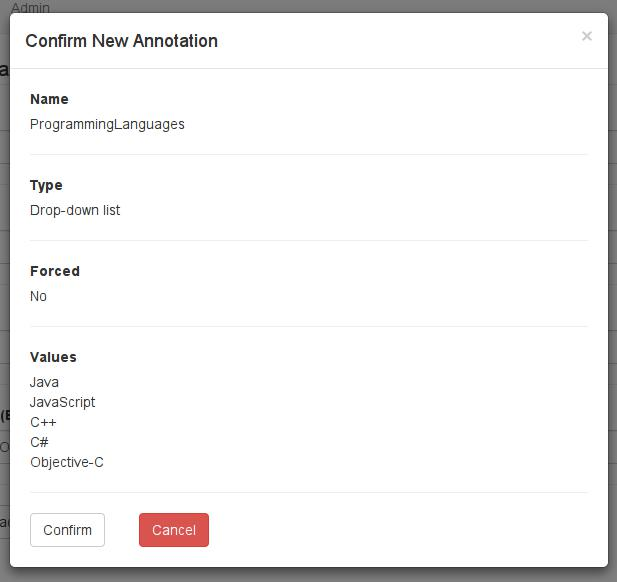
\includegraphics[width=0.7\textwidth]{web_SysadminCreateAnnotationConfirm.jpg}
 \caption{The confirm annotation pop-up.}
 \label{adm_web_createPopup}
\end{figure}



The example in \refer{adm_web_createPopup} will result in a drop-down annotation with the name Number of toes and possible values: 0, 1, 2, 3, 4, 5 with 0 as default and is not forced.

A back button which takes the user back to the annotations start page is also available in this view. In \refer{adm_web_createView} the create annotation view can be seen.

\begin{figure}[t]
 \addImage{web_SysadminCreateAnnotation.jpg}
 \caption{The view for administrators where new annotations can be created.}
 \label{adm_web_createView}
\end{figure}

The “Genome-releases” link on the sidebar takes the administrator to a page where it is possible to add and remove genome releases to and from the server (see \refer{adm_web_genomereleaseView}.

\begin{figure}[h]
 \addImage{web_SysadminGenomeReleaseView.jpg}
 \caption{The genome-release view.}
 \label{adm_web_genomereleaseView}
\end{figure}

The button “Select files to upload” opens the native file explorer where the user can select one ore multiple files and click on “OK”. This will open a popup-window, seen in \refer{adm_web_uploadconfirm}, showing what files that where chosen and asks for species and genome version before uploading. 

\begin{figure}[h]
 \centering
 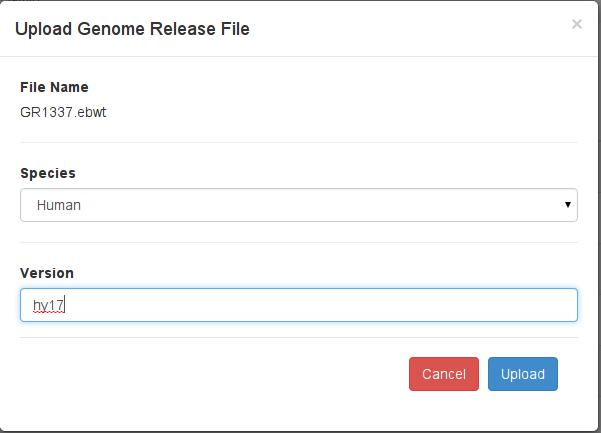
\includegraphics[width=0.7\textwidth]{web_SysadminUploadGenomeReleaseModal.jpg}
 \caption{Popup for uploading genome releases.}
 \label{adm_web_uploadconfirm}
\end{figure}

When the upload begins the popup closes and a progress-bar appears showing the progress, showing ''Upload completed'' when done. The user can at this stage move between pages without disturbing the upload but should not close or refresh the web browser. 

Every genome release in the table can be deleted by clicking on the “Delete” button next to the release. This will prompt a small popup asking for user confirmation and if given a positive response, deletes the genome release from the server and updates the view. 

If any genome release is used by an experiment already an error will appear telling the user exactly that. 

\subsection{Setting up the application}
To setup the application, move the content of the folder \url{genomizer-web/app/} to the desired location from where the application should be run. To run the web page, open a web browser and enter the url to the folder which contains the \class{index.html} file (where the content of app was placed).
For example, given that the \url{genomizer-web} folder is placed in the home folder of the Umeå university CS user \class{c11abc} and that user wants to put the web app in a folder called \url{public\_html/} which is also in the home folder of the user. In Linux, do the following steps:
\begin{enumerate}
	\item Navigate to the app folder: \texttt{“cd \textasciitilde /genomizer-web/app/”}
	\item Move the contents of app to the folder \url{public\_html}: \texttt{“mv * \textasciitilde /public\_html/”}
	\item Given that the url to \url{public\_html} is: \filePath{“www8.cs.umu.se/\textasciitilde c11abc/”}
	\item To run the application start a web browser and type \filePath{“www8.cs.umu.se/\textasciitilde c11abc/”}
\end{enumerate}
This will open the web page in the browser.

